\section{Description / Introduction}

Our project is based on the Freenove Three-Wheeled Smart Car Kit for Raspberry Pi. We use the hardware from the kit and follow the tutorial as a starting point, but we develop our own custom software to control the vehicle.
The kit includes a car frame, two wheels for steering and driving, a buzzer, an RGB light, a camera, and all necessary parts like screws and cables. It also comes with a special shield to control everything via a Raspberry Pi.

In addition, we use two lithium-ion batteries for power and a Raspberry Pi 4 to control the car.

We call our vehicle PiRover. It can be controlled through a Svelte-based web user interface. Communication with the PiRover works over Wi-Fi using MQTT and WebSockets. This allows us to send commands and receive data in real time.
Additionally, the camera’s live video feed is streamed to the web interface, allowing users to see the rover’s point of view.


\begin{figure}[h!]
    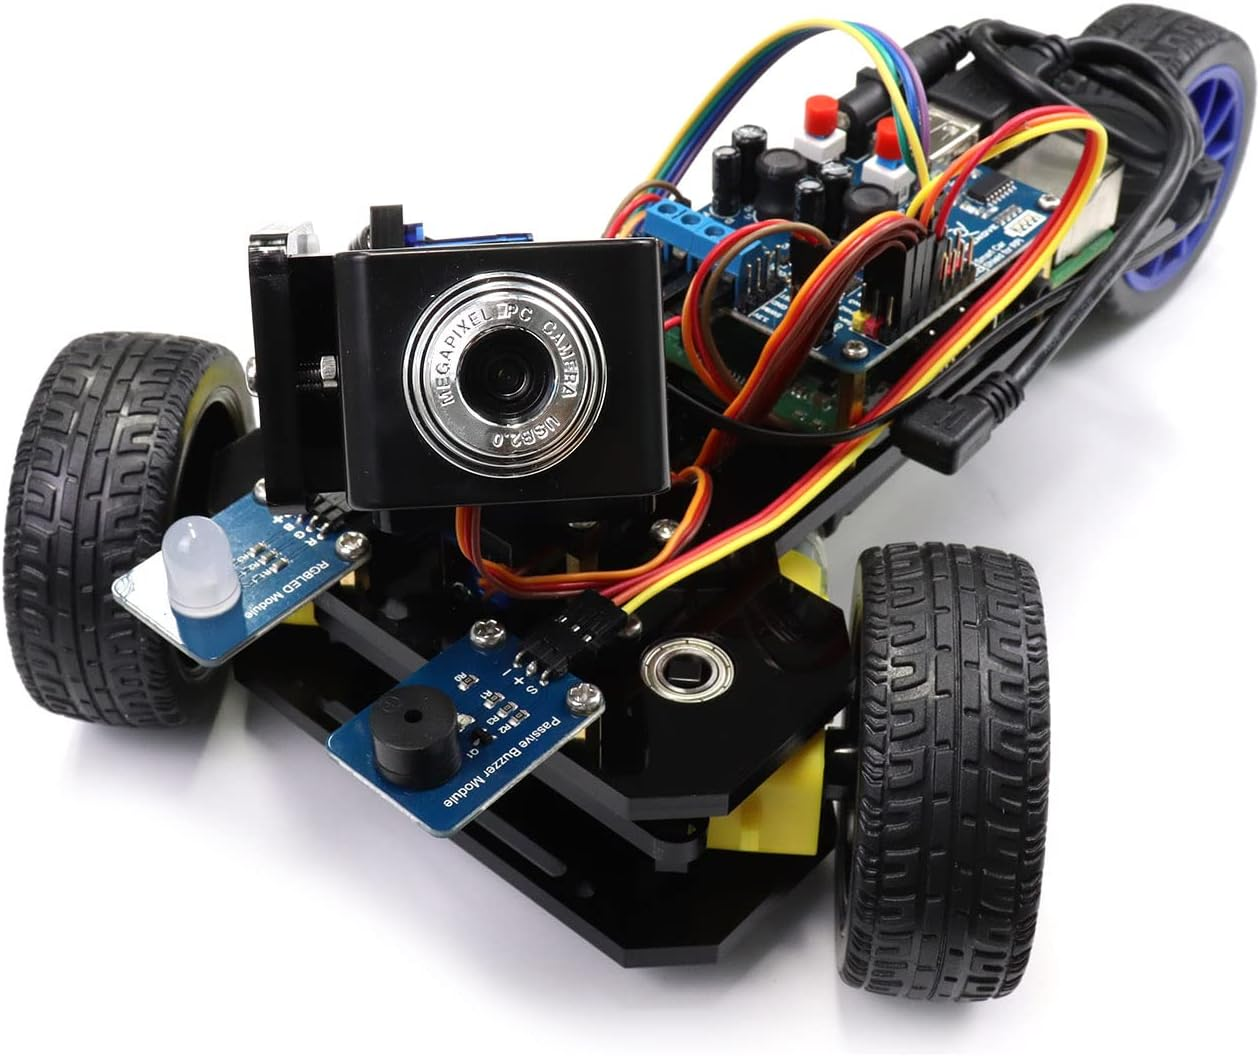
\includegraphics[width=15cm]{img/freenove_smartcar_imagepicture}
\end{figure}
